\graphicspath{{chapters/04_materials_and_methods/images/}}
\chapter{Materials and methods}

% The Materials and Methods section provides a detailed description of the protocols,
% software and algorithms used for the project (at least 3 pages, maximum 10 pages; if you need
% more pages, include an Appendix).

This chapter presents the HiCONA package, how it was implemented and what it can be used for. The main focus is on the steps leading to the creation of a network which can be then analyzed using standard or custom network analysis algorithms. One such algorithm, node-labels permutations, is then illustrated. The chapter does not explain how to actually use the package; for that, ample documentation and notebooks will be available as soon as the package will be made public.

\section{Implementation}
Hi-C Organization Network Analysis (HiCONA) is a \textbf{Python3 package} compatible with Python version 3.7 and later. The package strives to provide a fast, memory-efficient, flexible and user-friendly framework for network analysis of Hi-C data. In order to do so, it is implemented taking into account some key aspects:
\begin{itemize}\tightlist
  \item A fully \textbf{object-oriented programming} (OOP) approach is used to keep the functions organized and make it easy to extend with further functionalities.
  \item Well established file formats are used for both input and output, in order to facilitate package \textbf{integration} into already existing analysis pipelines.
  \item All expensive operations are \textbf{optimized} both in terms of memory usage and computational runtime, in such a way that almost any file can be quickly processed even on less performing systems such as laptops. This is mostly achieved by chunking and vectorizing operations.
\end{itemize}
HiCONA is mostly built on top of two main packages, those being \emph{cooler} and \emph{graph-tool}. \textbf{\emph{Cooler}} is a library designed to work with \texttt{.cool} files\cite{cooler2020}; from its Python API, HiCONA extends the main object class \texttt{Cooler} into \texttt{HiconaCooler}, which is responsible for data I/O, preprocessing and bin annotation. \textbf{\emph{Graph-tool}} is a Python package for network analysis\cite{graphtool2014}; it is highly optimized and fast since all algorithms and data structures are implemented in C++. The \texttt{Graph} object class from \emph{graph-tool} is extended into \texttt{HiconaGraph}, which is responsible for network manipulation and analysis. Other major packages HiCONA relies on are \emph{scipy}\cite{scipy2020} for integral computation, \emph{numpy}\cite{numpy2020} for algorithm implementation, \emph{pandas}\cite{pandas2020} for data manipulation, \emph{pybedtools}\cite{pybedtools2011} for bin annotation, \emph{seaborn}\cite{seaborn2021} and \emph{matplotlib}\cite{matplotlib2007} for plotting. Aside from the previously mentioned \texttt{HiconaCooler} and \texttt{HiconaGraph} classes, HiCONA also implements a \texttt{ChromTable} class to facilitate conversion among the two and some utility classes such as custom iterators for these object types.

\section{Package functionalities}
HiCONA implements everything which is needed to perform network analysis starting from a \texttt{.cool} file. As shown in the usage flowchart in figure \ref{fig:flowchart}, these functionalities can be roughly divided into three groups:
\begin{itemize}\tightlist
  \item \textbf{Pixel preprocessing}, which encompasses pixel filtering, normalization and sparsification, which allow to obtain chromosome-level tables ready to be converted into graphs, starting from the full contact matrix.
  \item \textbf{Bin annotation manipulation}, which includes adding bin annotations from bed-like files, deleting bin annotations or converting categorical bin annotations into one-hot encoding form.
  \item \textbf{Network generation and analysis}, which comprehends the creation of the graph object from the preprocessed chromosome-level pixel table and all the network analyses conducted on it.
\end{itemize} 

% TODO: Replace in image the placeholder pics
% TODO: Columns of last tables in part (a) of th epic are actually wrong

\begin{figure}
  \centering
  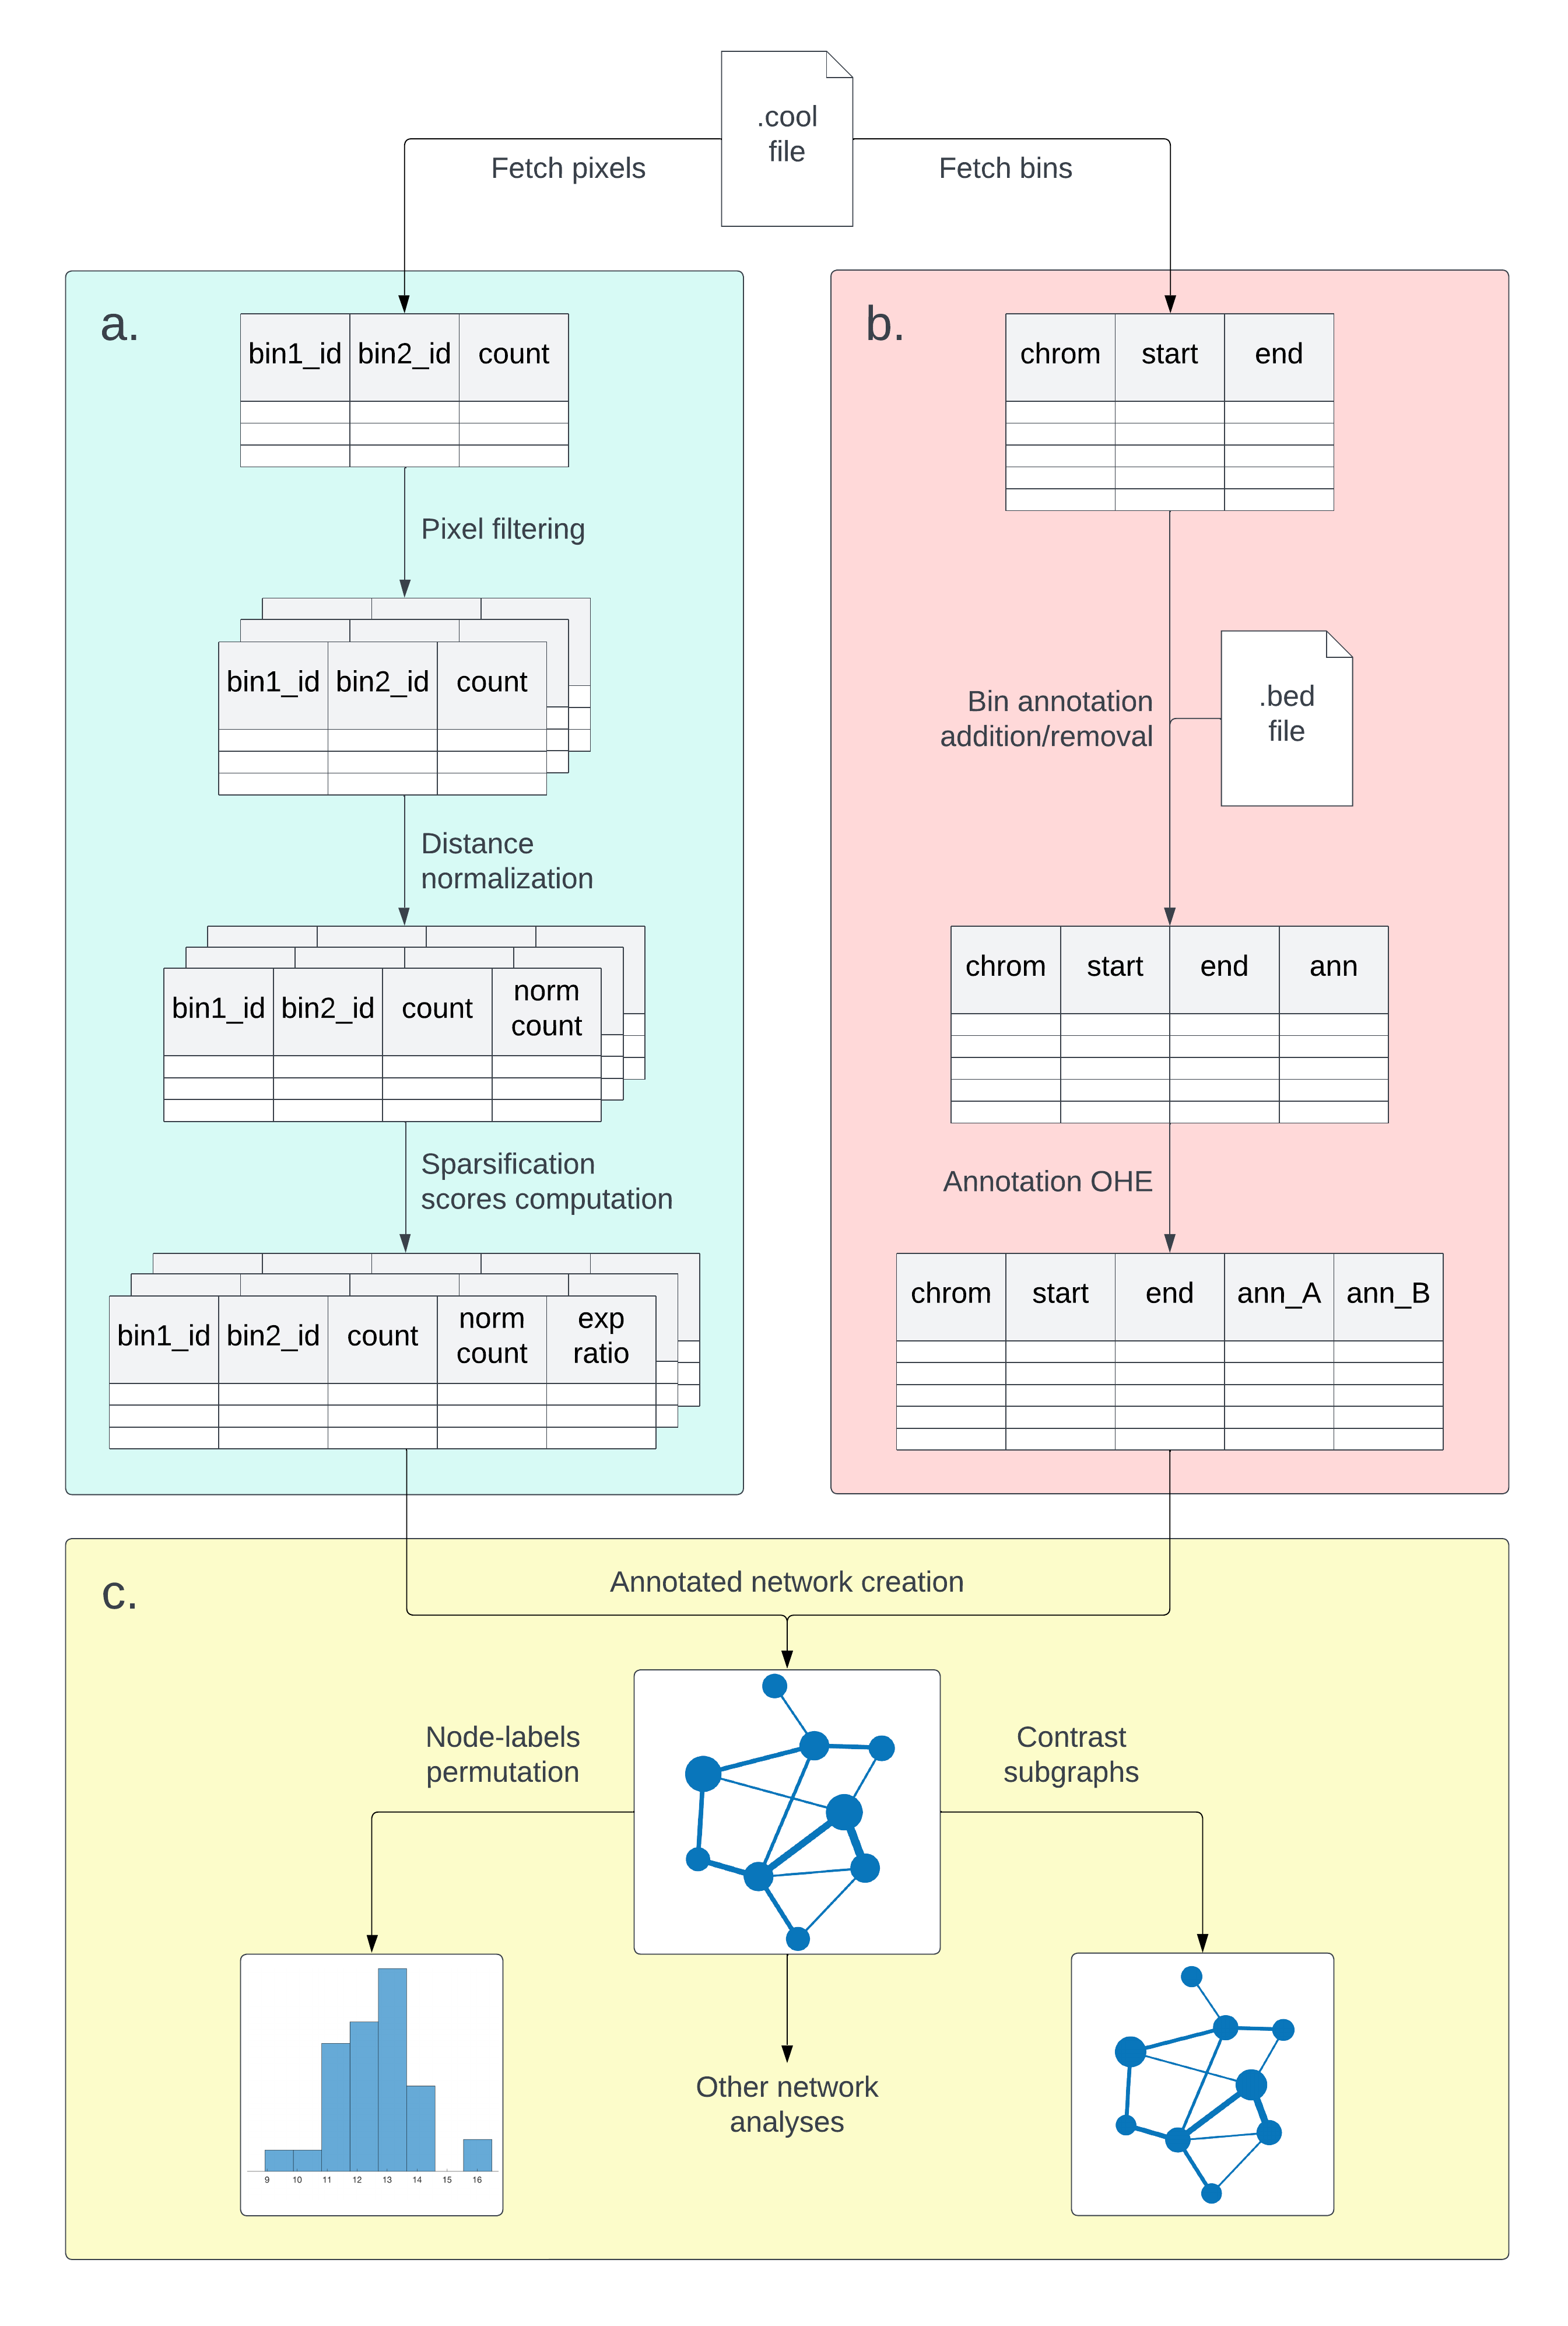
\includegraphics[width=0.85\textwidth]{package_flowchart.png}
  \caption{\textbf{HiCONA package flowchart}. Typical steps required for Hi-C data analysis using HiCONA. (a) Pixel preprocessing steps. Starting from the complete contact matrix, filter, normalize and compute the sparsification scores of the pixels. The end result is a reduced pixel table ready for conversion to network. (b) Bin annotation manipulation steps. All steps needed to add, remove or modify the optional bin annotation columns present in the file. (c) Network generation and analysis steps. Combine the prepared pixel table subsets with the bin annotations to create networks which can be analyzed with a multitude of algorithms.}
  \label{fig:flowchart}
\end{figure}

\section{Pixel preprocessing}
Pixel preprocessing includes all steps required to go from the full pixel table contained in a \texttt{.cool} file to one or more chromosome-level pixel tables, which are normalized subsets of the full table stored in the \texttt{.cool} file for later usage in network creation.  
Pixel preprocessing is a key step in order to be able to conduct downstream analyses, especially those requiring the comparison of different experiments and/or replicates. In order to guarantee consistent preprocessing, the procedure is fairly streamlined; all steps are handled by a single public method of the \texttt{HiconaCooler} class (\texttt{create\_tables}), to which the user can pass arguments if they want to supersede the default parameter values. For most applications, the default values should already be the optimal ones. If no default value is superseded, one chromosome-level pixel table for each chromosome will be created using those defaults. The preprocessing steps, described in the following subsections, are shown in the context of the usage flowchart in figure \ref{fig:flowchart} (a).

\subsection{Pixel filtering}\label{par:pixfiltering}

The initial preprocessing step is the retrieval and filtering of subsets of the pixels from the whole pixel table. For each specified chromosome (or all of them if no specific one is selected), a table containing all pixels whose first bin falls into that chromosome is created. Each of these tables is then filtered in order to remove:

\begin{itemize}\tightlist
  \item \textbf{Inter-chromosomal pixels}, meaning pixels whose bins do not fall into the same chromosome. This is the main simplifying step which allows to break the entire contact matrix into tables of manageable size; moreover, inter-chromsomal pixels are removed since they also constitute a problem for genomic distance normalization (see the following subsection).
  \item \textbf{Self-looping pixels}, meaning pixels whose bins are identical (main diagonal of the contact matrix). Self-looping pixels can exist since the two sequences constituting the sequencing read in the Hi-C experiment are typically way shorter than the bin size, and can therefore fall into the same bin. These pixels are removed since the contact frequency is too variable, leading to very noisy signal.
  \item Pixels whose bins have a \textbf{genomic distance} among them \textbf{above a certain threshold}; this correspond to removing the pixels where the bins are so far apart that is likely that the contact is random and not biologically significant. Currently, the default value for this distance is 200 Mb.
  \item Optionally, pixels whose count value is lower than a threshold; this can be used to speed up computation in less performing systems, but it should be avoided if possible since it introduces instability during distance normalization and most pixels with very low counts are removed during network sparsification anyway.
\end{itemize}

Notice that, the way the initial subsetting is performed, not all inter-chromosomal pixels are fetched, specifically not those where the bin belonging to the chromosome of interest is the second in the pixel; this does not matter currently, since inter-chromosomal pixels are filtered out anyway. 

As of now, subsetting is supported only at chromosome-level and this is because subsetting on arbitrary genomic coordinates would lead to some issues. Even though the preprocessing procedure would work without issues (given that it is chunked), subsetting on a region larger than a chromosome could lead to extremely big networks downstream which would be difficult to handle; moreover, unless the inter-chromosomal filter is removed, the two chromosomes would be disconnected anyway. On the other hand, subsetting on a region smaller than a chromosome would skew the sparsification procedure, since it would arbitrarily remove some connections of the bins. Arbitrary subsetting might be added in the future if a compelling reason is found.

\subsection{Pixel distance normalization}\label{par:distnorm}
% TODO: Maybe say why HiCONA does not perform systematic bias normalization. PROBABLY JUST EXPLAIN THAT THE GENOMIC DISTANCE IS BY FAR THE HIGHEST CAUSE FOR CONTACT NUMBERS. MOREOVER DIFFICULT TO NORMALIZE IN GC CONTENT IF THE REGION IS FAIRLY BIG.

A very important notion to keep into account, while preprocessing this type of data, is pixel genomic distance, which is the \textbf{genomic distance} among the two bins composing the pixel. Formally, this can be defined as 
$$d_i = r(b_{2i} - b_{1i})$$
where $d_i$ is the genomic distance for pixel $i$, $b_{2i}$ and $b_{1i}$ are the bin ids for the second and first bins of that pixel, $r$ is the working resolution, meaning a positive integer representing bin size in bp. It is known that the probability of random contact among two bins exponentially decays with the genomic distance among them\cite{distancedecay2009}; this means that pixels whose bins are closer to each other will tend to have significantly higher counts with respect to pixels whose bins are further away just due to random chance. This in turn translates into the fact that, without some correction for this bias, potentially meaningful long range interactions will be outshadowed by random close range interactions. The most natural way to perform this type of normalization is to rescale the counts using some summary statistic which is a function of genomic distance ($P(d)$).

Although not directly for normalization purposes, the \texttt{cooltools} package\cite{cooltools2022} can compute one such summary statistic for intra-chromosomal pixels, that being the expected counts given a genomic distance. Formally speaking, it can be defined as
$$P\left(d\right) = \frac{\sum_{i=1}^n c_i \cdot I(d = d_i)}{\sum_{i=1}^n I(d = d_i)}$$
where $c_i$ is the count value of the $i$-th pixel, $n$ is the total number of pixels, and $I$ is an indicator function (1 if the genomic distance of the $i$-th pixel is the same as the one of interest, 0 otherwise). From a graphical point of view it corresponds to averaging the count values of all pixels on the same diagonal of the contact matrix. In reality the algorithm is slightly more complex, working on individual chromosome arms and removing some regions such as telomeres and centromeres. Since at high genomic distances the number of averaged pixels becomes progressively smaller, the expected counts estimates become more and more unstable; for this reason \texttt{cooltools} can perform a smoothing of the expected counts by distance curve by averaging the values in a sliding window of increasing size (basically, use the fact that very similar distances should have only a slight difference in expected counts). 
This method is straight forward and immediate to understand, yet it has a major downside when used for normalization purposes: all pixels at a given distance are considered, even those with count value equal to zero, and given that these zero-count pixels are the majority of pixels, especially at high genomic distances, the expected counts quickly tend to zero. Extremely small values are difficult to use for normalization purposes, since they cannot be used as fraction denominator, otherwise the values would explode.
% TODO: Talk more about instability at high distance if needed to fill space
% TODO: Consider adding an image to make things more clear

For this reason, HiCONA proposes a slightly different approach to compute the \textbf{summary statistic} for normalization purposes: only non-zero count pixels are considered and the median value is taken for each distance rather than the mean. Formally, this can be written as:
$$P\left(d\right) = median(\{c_i|(d_i=d) \land (c_i \neq 0) \, \forall i \in [1,n]\})$$ 
where $\{\}$ represents a multiset (set with multiplicity).
Notice that this means that the normalization factors will always be positive integers, therefore solving the denominator issue. Once the $P(d)$ curve has been computed, the \textbf{normalized count value} for the $i$-th pixel can be computed as
$$m_i = \log_2 \left(\frac{c_i}{P(d_i)} + 1\right)$$
where $m_i$ is the normalized count value, $c_i$ is the count value for that pixel and $P(d_i)$ is the normalization factor corresponding to the genomic distance of that pixel. Even though the normalized count value is a floating point number, it is derived from a fraction of two integers which can take a fairly limited number of values (especially the denominator); for this reason, the number or actual values that the normalized counts can take is relatively small, allowing the usage of memoization in later steps to speed up computations.

Optionally, the user can specify a percentile as filter; all pixels whose normalized counts fall below the specified percentile are removed. This is done to both remove some noise as well as reduce dimensionality. 
 
All considerations up till this point are applicable only to \textbf{intra-chromosomal pixels}. This is because it is not possible to define a notion of genomic distance for inter-chromosomal ones. Still, \texttt{cooltools} does give the option of computing the expected counts for inter-chromosomal pixels; given a pair of chromosomes, the expected counts are given by the average of all pixels counts where one bin belongs to one chromosome and one bin belongs to the other. HiCONA could implement a similar method for inter-chromosomal pixel normalization but it currently does not. This is because, ultimately, the normalized values are used to compute the edge weights; if both inter and intra-chromosomal pixels were to be kept, the network would contain edges whose weights were computed using different procedures, and therefore there would not be a way to guarantee that the comparison is fair. For this reason, and those listed previously, all inter-chromosomal pixels are removed.

\subsection{Pixel sparsification score computation}\label{par:sparscore}

The normalized chromosome-level pixel tables could already be converted into networks; that being said, the resulting networks would be rather big in size (about $7 \cdot 10^7$ edges) and noisy (many edges with very low weight). In order to mitigate this problems, a network sparsification algorithm\cite{sparsification2009} is used; the objective of the procedure is to sparsify the network, i.e. reducing graph density (the number of edges in the graph), while retaining most of the overall topological properties and structure of the network.

While standard top-n edge filtering keeps only the top $n$ scoring edges according to their weight, network sparsification keeps the edges which are contributing the most in defining the first order neighbourhoods of the nodes in the graph. This means that edges with relatively low weight but very high contribution in defining the local structure of the network are kept using network sparsification, while they would not be using top-n edge filtering. This is important when trying not to belittle nodes with lower strength.

The algorithm, shown fully in Alg.\ref{alg:originalSparsification}, can be summarized as follows. For each edge $ij$ in the graph, tangent to the nodes $i$ and $j$, two sparsification alpha scores are computed, one for each tangent node ($\alpha_{ij,i}$ and $\alpha_{ij,j}$ respectively); using node $i$ as an example, the sparsification score would be computed as
$$\alpha_{ij,i} = 1 - (k_i-1) \int_0^{p_{ij,i}}(1-x)^{k_i-2}dx$$
where $k_i$ is the number of neighbours of node $i$ and $p_{ij,i}$ is the normalized edge weight for edge $ij$ considering the neighbourhood of $i$, which means 
$$p_{ij,i} = \frac{w_{ij}}{s_i}$$ 
with $w_{ij}$ being the weight of edge $ij$ and $s_i$ being the strength of node $i$ (both of which distance normalized). The value $\alpha_{ij,i}$ represents the probability (or p-value) of edge $ij$ having weight $w_{ij}$ assuming random distribution of edge weight among all neighbours of node $i$.
The same procedure is repeated for node $j$.
After computing both $\alpha_{ij,i}$ and $\alpha_{ij,j}$, only one value is kept for each edge, generally the minimum of the two
$$\alpha_{ij} = \min(\alpha_{ij,i}, \alpha_{ij,j})$$
After having computed $\alpha_{ij}$ for every edge, the graph can be sparsified by removing all edges whose sparsification score is below a certain threshold $\alpha$
$$\text{keep edge } ij \iff \alpha_{ij} < \alpha$$

\begin{algorithm}[h]
\setstretch{1.15}
\caption{Network sparsification algorithm, Serrano et. al, 2009}\label{alg:originalSparsification}
\begin{algorithmic}[1]
\Require $G$ = a weighted, undirected graph defined over vertices $V$ and edges $E$, $\alpha$ = sparsification cutoff
\Ensure $G'$ = the sparsified graph
\Statex
\State \textbf{Step 1: sparsification score computation}
\State Set $\alpha_{ij, curr} = 1, \forall (i,j) \in V, j \in \text{neighbours of } i$ \,\, (Note: $\alpha_{ij} = \alpha_{ji}$ since $G$ is undirected)
\For{$i \in V$}
    \State $w_{sum} =$ sum of the weights of all edges incident to $i$
    \State $k_i =$ degree of node $i$ 
    \For{$j \in$ neighbours of $i$} 
      \State $w_{norm} = w_{ij} / w_{sum}$
      \State $\alpha_{ij, new} = 1 - (k_i-1) \int_0^{w_{norm}}(1-x)^{k_i-2}dx$
      \State $\alpha_{ij, curr} = \min(\alpha_{ij, curr},\alpha_{ij, new})$
    \EndFor
\EndFor
\Statex
\State \textbf{Step 2: network filtering}
\State $G' =$ empty graph
\For{$e_{ij} \in E$}
    \If{$\alpha_{ij, curr} < \alpha$}
        \State Add edge $e_{ij}$ to $G'$
    \EndIf
\EndFor
\end{algorithmic}
\end{algorithm}

Some considerations to be made regarding this algorithm: 
\begin{itemize}\tightlist
  \item If the number of neighbours is 1, then the alpha score will always be 1. This means that, for an edge tangent to a terminal node, the sparsification score derived from the non-terminal node will always be chosen, since it will always be less than, or equal to, 1. Moreover, if both nodes tangent to an edge are terminal, meaning that they form a disconnected component of two nodes (\emph{doublet}), the edge will always have sparsification score equal to 1 and thus the edge will always be removed regardless of the threshold used. This is fine since a disconnected doublet is not very informative for network analysis purposes.
  \item Given that the sparsification alpha values are p-values, they always take a value in the range $(0,1]$. Moreover, given that they are p-values, one might expect multiple correction testing to be needed; this is not the case, given the fact that the main objective is not to filter out the significant edges, but rather to denoise and try to reconduct the network to a somewhat standard and reproducible form usable for comparison. For the same reason, the alpha cutoff is not necessarily the standard 0.05 generally used for p-values, and even in the original sparsification paper other values are suggested and used.
  \item HiCONA also allows to choose the maximum of the two sparsification scores, since they have different meaning. Choosing the minimum means that the edge will be kept if it is significant for at least one node; on the contrary, choosing the maximum would mean keeping the edge only if significant for both nodes. Using the minimum can be seen as the more conservative options, while using the maximum yields a less noisy graph though at the expense of some potentially relevant weak edges.
\end{itemize}

HiCONA does not directly sparsify the network, but rather stores the sparsification scores for a later use; by deferring network filtering, one can generate networks using different cutoffs without having to recompute the scores. HiCONA does allow filtering according to any arbitrary threshold; for this reason one might want to use a fixed value as cutoff, for instance 0.05. However, one such value is, indeed, arbitrary and does not necessarily meet the need for comparable graphs. For this reason the package can compute a graph-dependent threshold, defined as the value which maximizes the fraction of retained nodes (nodes that are still tangent to at least one edge after the filtering) while also minimizing the fraction of edges in the graph. To do so, multiple thresholds are tested and the one with the smallest Euclidean distance from the point $(1,0)$, in the plane with the fraction of retained nodes on the x-axis and the fraction of retained edges on the y-axis, is chosen.

The network sparsification procedure is quite simple to apply, assuming that the entirety of the data can be loaded into memory either in a dense adjacency matrix or in a graph-like structure. While the former is not an option due to the previously discussed nature of Hi-C data, a graph can be reasonably generated, though the amount of memory required might be quite prohibitive if a server is not being used. The algorithm could be thus modified to work with chunks of the graph rather than the entirety of it, though this is non-trivial considering that the data is in $ijv$ form. For this reason, HiCONA implements a modified version of the algorithm which works on chunk of the $ijv$ table; though the modified algorithm has a slightly higher complexity, requiring more passes of the pixels, it allows to work at a fixed RAM-footprint specified by the user, making it possible to be used even on laptops. Moreover, the modified version is easy to vectorize and it is therefore quite fast (and it could be sped up even more using parallelization).

\section{Bin annotation manipulation}

The cooler format is structured in order to accommodate for any number and type of bin annotations, and in fact most \texttt{.cool} files have a some bin normalization weight column by default. Although this is the case, the \emph{cooler} package does not provide a very convenient facility to manipulate these annotations; for this reason HiCONA does implement methods to add, remove and manipulate bin annotations, which are shown in figure \ref{fig:flowchart} (b). 

\subsection{Adding and removing bin annotations}

HiCONA allows to add annotations to the bin table of the \texttt{.cool} file starting from a bed-like file. To be more precise, the package uses \emph{pybedtools} to perform a left outer join of the bin table and the bed-like file. The user can then decide to keep any number of columns from the bed-like file to use as annotations; moreover, a binary annotation column can be created, containing 1 if the bin has any overlap with any interval in the bed-like file. Currently any number of overlapping bases greater than zero is considered enough for bin annotation.

HiCONA does allow removing bin annotations by specifying the name of the annotation to be removed; however, currently, removing an annotation does not reduce file size. This is due to how \texttt{.hdf5} files work since, rather than removing a dataset, they remove its memory address pointer so that it cannot be reached anymore (this is to avoid having to shift the position of the other bytes in memory and reindexing). To reduce file size after removing an annotation, an external tool such as \emph{h5repack} can be used, though this functionality might be added natively in the future.

\subsection{Bin annotation OHE}

Working with a categorical bin annotation with multiple modalities is not convenient, especially for algorithms such as node-labels permutations. For this reason, HiCONA allows to convert any categorical bin annotation to One Hot Encoding (OHE). This means that, given a categorical annotation, for each modality of that annotation a new binary annotation is created, where 1 indicates that the bin was annotated as that modality, 0 otherwise. For example, the annotation $ann=[A,B,A,A]$ would be split into $ann\_A=[1,0,1,1]$ and $ann\_B=[0,1,0,0]$. A hard cap is placed on the number of modalities an annotation can have and be split, in order to prevent splitting annotations such as gene names into thousands of columns.

\section{Network generation and analysis}

After the chromosome-label pixel tables have been created, and any required annotation has been added to the bin table, the networks are ready to be generated and analyzed. The minimal network is created by selecting a pixel table to use as edge list; unless otherwise specified, the edges are then annotated with raw counts, normalized counts and sparsification score, while the nodes are annotated with the corresponding bin id, chromosome, start and end. Any number of other node annotations can be also added, provided that it is present in the bin table. Moreover, a sparsification score cutoff can be specified to filter the edges prior to building the network.

Once a network, which is an instance of the \texttt{HiconaGraph} class, has been created, it can be analyzed either with one of the many generic network analysis algorithms inherited from the \emph{graph-tool} package, or using one of the more specific algorithms implemented by HiCONA. Currently HiCONA only implements node-labels permutation, while contrast subgraphs extraction is being developed (both shown in figure \ref{fig:flowchart} (c)), but the package is structured in such a way that it can be easily extended to accommodate other analysis algorithms.

\subsection{Node-labels permutation}

Node-labels permutation, or simply node permutation, is a widely used algorithm in network science; its main objective is to test whether the average (or distribution) of some node-level statistic differs among nodes with different labels (bin annotations). As an example on Hi-C data, one might want to test whether bins containing a promoter region tend to form more connections, on average, with respect to bins containing a boundary region. 

The algorithm, displayed in Alg.\ref{alg:labelPermutations}, can be summarized as follows. A network, whose nodes are annotated as either $A$, $B$, none or both, is given; $A$ and $B$ are the two labels which are to be compared. Once some node-level statistic has been defined, that statistic is computed for all nodes annotated as $A$ and then averaged. After this has been repeated for the nodes annotated as $B$, the $\log_2$ fold change among the two is computed; this is the \emph{original} fold change. Then, an empirical distribution is created by randomly shuffling node annotations and recomputing the fold change for $N$ times, where $N$ is the number of specified permutations; notice that the actual structure of the network never changes. The fraction of \emph{permuted} fold changes which are more extreme (higher) than the \emph{original} fold change is the p-value for the test $H_0: S(A) \leq S(B), \, H_1: S(A) > S(B)$, where $A$ and $B$ represent the sets of nodes annotated as $A$ and $B$, respectively, and $S$ is the average statistic for a node set. 

\begin{algorithm}
\setstretch{1.15}
\caption{Node-labels permutation algorithm}\label{alg:labelPermutations}
\begin{algorithmic}[1]
\Require $G$ = a graph defined over vertices $V$ and edges $E$; each vertex can be annotated as $A$, $B$, both or neither. $S$ = the average of a node-level statistic over a set of nodes. $N$ = the number of permutations to perform.
\Ensure The p-value for the test $\begin{cases} H_0: S(A) \leq S(B) \\ H_1: S(A) > S(B) \end{cases}$
\State Define a vector of node labels $L = \left[l_1, l_2, \dots, l_{|V|}\right]$, such that each element is a tuple $l_i = (l_{Ai}, l_{Bi})$ with $l_{Ai} = 1$ if $v_i$ is annotated as $A$, 0 otherwise (define $l_{Bi}$ analogously)
\State Define the sets $A = \{v_i | v_i \in V, l_{Ai} = 1\}$, $B = \{v_i | v_i \in V, l_{Bi} = 1\}$
\State Compute $s_{original} = \log_2(S(A)/S(B))$
\State Initialize $counter = 0$ 
\For{$n \in [1, N]$}
    \State $L_n = [l_{\pi_n(1)}, l_{\pi_n(2)}, \dots, l_{\pi_n(|V|)}]$, where $\pi_n$ is some permutation function
    \State $A_n = \{v_i | v_i \in V, l_{n, Ai}=1\}$, $B_n = \{v_i | v_i \in V, l_{n, Bi}=1\}$
    \State $s_{permutation} = \log_2(S(A_n)/S(B_n))$
    \If{$s_{permutation} > s_{original}$}
        \State $counter = counter + 1$
    \EndIf
\EndFor
\State $p_{val} = (counter + 1) / (N + 1)$
\end{algorithmic}
\end{algorithm}

The annotations which can be used for this algorithm are all those added to the bin table, as long as they were converted to OHE. Moreover, HiCONA can assign the mock label \emph{universe} to all nodes in the network, which allows to compare nodes with a specific label with respect to the entire network.

Like any statistical test which has to be applied multiple times, some p-value correct should be applied, such as the \emph{Benjamini-Hochberg} correction. This is because the procedure is likely to be repeated for all chromosomes, for multiple pairs of annotations and possibly for multiple resolutions, therefore leading to some hundreds of tests. Currently HiCONA does not natively apply any correction.

Different node level statistics can be used, with different meaning at the network level. Some statistics that can be used, and which are implemented in HiCONA, are degree, betweenness centrality and local clustering coefficient. For in depth explanation of their definition and meaning, refer to Appendix I.


\section{Benchmarking}

In this section, both files and methods used to benchmark memory and runtime of the tool are presented. Benchmarking was performed only on the preprocessing steps, given that they are the limiting factors in term of performance.

\subsection{Memory and runtime benchmarking}

Given the focus of the package on being fast and usable even on less performing systems, benchmarking on both RAM usage and computational runtime are needed. This is especially true for the preprocessing part, when data dimensionality is still very high.

Memory benchmarking is performed through the \emph{memory\_profiler}\cite{memprof} Python package.
To display RAM usage line-by-line, the functions to profile must be preceded by the \emph{@profile} decorator, then the code can be run to generate a log-like file. The package also allows to display RAM usage overtime, however the default package plotting functions have been substituted with custom ones for better clarity.

Since runtime benchmarking was performed only on the preprocessing steps, none of which are parallelized yet, wall time was used rather than CPU time, in order to have an estimate from a more practical point of view. Computational runtime benchmarking was performed simply using the built-in \emph{timeit} module.

\subsection{Test datasets}

Several datasets have been used for benchmarking purposes, all of which are available on the 4D Nucleome data portal\cite{4dn2022}. Although those datasets are available as \texttt{.mcool} files, due to a bug during file generation (confirmed by the database maintainers), the \texttt{.cool} files had to be re-generated starting from the \texttt{.pairs.gz} files using \emph{pairix}\cite{pairix2022} and
\emph{cooler}. The datasets were analyzed at the 5 kb and 10 kb resolutions; this is because these bin sizes are a good compromise in terms of having high enough detail while still working with contact matrices which are not exceedingly sparse. For each dataset, rather than file size, the number of pixels is reported; this is because the actual number of pixels is a better proxy for how the algorithms will scale, considering that: 
\begin{itemize}\tightlist
  \item The pixel table will always be some orders of magnitude bigger than the bin table; for instance, the 10 kb bin table for a human cell line file will have around $3 \times 10^5$ rows (constant number depending on genome size), while an average pixel table will have around $1.5 \times 10^9$ rows (variable number depending mostly on experiment coverage and number or replicates merged to create the file).
  \item Total file size takes into account bin annotations, which can take a huge amount of space (especially when categorical with many modalities, such as names, since they have to be stored as strings) and do not impact preprocessing run time.
\end{itemize}

The procedure was tested on data coming from different cell lines processed with the same restriction enzyme, as well as on data coming from the same cell line processed with different restriction enzymes. This is to start testing whether cell type and restriction enzyme introduce noticeable bias; still, a more in depth analysis, with multiple files per combination of cell type and restriction enzyme, would be needed for a definite answer to this question. For two cell types, GM12878 and IMR90, the biological and technical replicates, which were merged to obtain the full-size files, are also analyzed individually; this is to test how reproducible the procedure is on replicates, as well as how similar the processed full-size files are to the processed individual replicates. This last point is of particular interest since a high concordance would mean that the same results could be obtained by performing less experiments and sequencing, reducing costs for a technique which is rather expensive. 

The package is designed to work with \texttt{.cool} files as input, since the main objective is the analysis of Hi-C data; still, any type of data representable in \texttt{.cool} format can be analyzed, therefore the package has also been tested on a data file coming from another technique, namely Micro-C.

The characteristics of the analyzed datasets are summarized in Table \ref{datasets_table}.

\begin{table}[h]
\begin{center}
\begin{tabular}{|ccccccc|}
\hline
\multicolumn{1}{|c|}{4DN ID} &
  \multicolumn{1}{c|}{Publication} &
  \multicolumn{1}{c|}{Experiment} &
  \multicolumn{1}{c|}{Enzyme} &
  \multicolumn{1}{c|}{Cell Type} &
  \multicolumn{1}{c|}{Res (kb)} &
  Pixels \\ \hline
\rowcolor[HTML]{EFEFEF} 
\cellcolor[HTML]{EFEFEF} &
  \cellcolor[HTML]{EFEFEF} &
  \cellcolor[HTML]{EFEFEF} &
  \cellcolor[HTML]{EFEFEF} &
  \cellcolor[HTML]{EFEFEF} &
  5 &
  $1.89 \cdot 10^9$ \\
\rowcolor[HTML]{EFEFEF} 
\multirow{-2}{*}{\cellcolor[HTML]{EFEFEF}4DNFIYECESRC} &
  \multirow{-2}{*}{\cellcolor[HTML]{EFEFEF}Rao, 2014} &
  \multirow{-2}{*}{\cellcolor[HTML]{EFEFEF}In situ Hi-C} &
  \multirow{-2}{*}{\cellcolor[HTML]{EFEFEF}MboI} &
  \multirow{-2}{*}{\cellcolor[HTML]{EFEFEF}GM12878} &
  10 &
  $1.57 \cdot 10^9$ \\
 &
   &
   &
   &
   &
  5 &
  $4.95 \cdot 10^8$ \\
\multirow{-2}{*}{4DNFIIG4IWKW} &
  \multirow{-2}{*}{Rao, 2014} &
  \multirow{-2}{*}{In situ Hi-C} &
  \multirow{-2}{*}{MboI} &
  \multirow{-2}{*}{IMR90} &
  10 &
  $4.03 \cdot 10^8$ \\
\rowcolor[HTML]{EFEFEF} 
\cellcolor[HTML]{EFEFEF} &
  \cellcolor[HTML]{EFEFEF} &
  \cellcolor[HTML]{EFEFEF} &
  \cellcolor[HTML]{EFEFEF} &
  \cellcolor[HTML]{EFEFEF} &
  5 &
  $2.15 \cdot 10^8$ \\
\rowcolor[HTML]{EFEFEF} 
\multirow{-2}{*}{\cellcolor[HTML]{EFEFEF}4DNFIIFAUT24} &
  \multirow{-2}{*}{\cellcolor[HTML]{EFEFEF}Rao, 2014} &
  \multirow{-2}{*}{\cellcolor[HTML]{EFEFEF}In situ Hi-C} &
  \multirow{-2}{*}{\cellcolor[HTML]{EFEFEF}MboI} &
  \multirow{-2}{*}{\cellcolor[HTML]{EFEFEF}HMEC} &
  10 &
  $1.83 \cdot 10^8$ \\
 &
   &
   &
   &
   &
  5 &
  $2.00 \cdot 10^8$ \\
\multirow{-2}{*}{4DNFIYL35EHL} & 
  \multirow{-2}{*}{Rao, 2014} &
  \multirow{-2}{*}{In situ Hi-C} &
  \multirow{-2}{*}{MboI} &
  \multirow{-2}{*}{HUVEC} &
  10 &
  $1.77 \cdot 10^8$ \\


\rowcolor[HTML]{EFEFEF} 
\cellcolor[HTML]{EFEFEF} &
  \cellcolor[HTML]{EFEFEF} &
  \cellcolor[HTML]{EFEFEF} &
  \cellcolor[HTML]{EFEFEF} &
  \cellcolor[HTML]{EFEFEF} &
  5 &
  $1.41 \cdot 10^8$ \\
\rowcolor[HTML]{EFEFEF} 
\multirow{-2}{*}{\cellcolor[HTML]{EFEFEF}4DNFIUTE4F4B} &
  \multirow{-2}{*}{\cellcolor[HTML]{EFEFEF}Oksuz, 2021} &
  \multirow{-2}{*}{\cellcolor[HTML]{EFEFEF}In situ Hi-C} &
  \multirow{-2}{*}{\cellcolor[HTML]{EFEFEF}HindIII} &
  \multirow{-2}{*}{\cellcolor[HTML]{EFEFEF}H1-hESC} &
  10 &
  $1.26 \cdot 10^8$ \\
 &
   &
   &
   &
   &
  5 &
  $8.91 \cdot 10^7$ \\
\multirow{-2}{*}{4DNFIUPGJLFO} &
  \multirow{-2}{*}{Oksuz, 2021} &
  \multirow{-2}{*}{In situ Hi-C} &
  \multirow{-2}{*}{DpnII} &
  \multirow{-2}{*}{H1-hESC} &
  10 &
  $7.41 \cdot 10^7$ \\
\rowcolor[HTML]{EFEFEF} 
\cellcolor[HTML]{EFEFEF} &
  \cellcolor[HTML]{EFEFEF} &
  \cellcolor[HTML]{EFEFEF} &
  \cellcolor[HTML]{EFEFEF} &
  \cellcolor[HTML]{EFEFEF} &
  5 &
  $8.16 \cdot 10^7$ \\
\rowcolor[HTML]{EFEFEF} 
\multirow{-2}{*}{\cellcolor[HTML]{EFEFEF}4DNFIPVA6VYB} &
  \multirow{-2}{*}{\cellcolor[HTML]{EFEFEF}Oksuz, 2021} &
  \multirow{-2}{*}{\cellcolor[HTML]{EFEFEF}In situ Hi-C} &
  \multirow{-2}{*}{\cellcolor[HTML]{EFEFEF}DdelI} &
  \multirow{-2}{*}{\cellcolor[HTML]{EFEFEF}H1-hESC} &
  10 &
  $7.41 \cdot 10^7$ \\
 &
   &
   &
   &
   &
  5 &
  $5.73 \cdot 10^7$ \\
\multirow{-2}{*}{4DNFIR1FK55F} &
  \multirow{-2}{*}{Oksuz, 2021} &
  \multirow{-2}{*}{Micro-c} &
  \multirow{-2}{*}{MNase} &
  \multirow{-2}{*}{H1-hESC} &
  10 &
  $4.39 \cdot 10^7$ \\ \hline
\end{tabular}
\caption{\textbf{Summary of the datasets used for benchmarking}. Table summarizing the characteristics of the analyzed datasets. From left to right: 4DNucelome Data Portal id of the .pairs file converted to .cool, reference publication, experiment type, restriction enzyme used for DNA fragmentation, cell type, resolution (bin size) in kilobases, number of pixels in the file.}
\label{datasets_table}
\end{center}
\end{table}
